% Capital Allocation II -- factor bets and alpha bets. The same formula on hedged portfolios, and where the alphas come from.
% Figures and every number quoted here come from capital_allocation_figures.py
% Companion notebook: chapters/Finance/L12b_CapitalAllocationII_v2_AI.ipynb (parts 1-3 in class, the challenge is homework)
\documentclass[aspectratio=169,10pt]{beamer}
\usetheme{default}
\usecolortheme{default}

\usepackage{graphicx}
\usepackage{adjustbox}
\usepackage{amsmath}
\usepackage{amssymb}
\usepackage{booktabs}
\usepackage{array}
\usepackage{tikz}
\usetikzlibrary{arrows.meta,positioning,calc,decorations.pathreplacing}
\usepackage{appendixnumberbeamer}  % Exclude appendix from slide count

\setbeamertemplate{navigation symbols}{}
\setbeamertemplate{items}[circle]

% Footline: Author, Event (Year) on left; page/total on right
\setbeamertemplate{footline}{
  \hbox{%
    \begin{beamercolorbox}[wd=.5\paperwidth,ht=2.5ex,dp=1ex,left]{author in head/foot}%
      \hspace*{2ex}\insertshortauthor, \insertshortinstitute\ (\insertdate)
    \end{beamercolorbox}%
    \begin{beamercolorbox}[wd=.5\paperwidth,ht=2.5ex,dp=1ex,right]{date in head/foot}%
      \insertframenumber/\inserttotalframenumber\hspace*{2ex}
    \end{beamercolorbox}%
  }
}

% Highlight boxes
\setbeamercolor{box1}{bg=red!12,fg=black}

% A poll option: {colour}{letter and choice}
\newcommand{\pollbox}[2]{\tikz\node[draw=#1!65!black, fill=#1!10, rounded corners=4pt, minimum width=3.7cm,
                                   minimum height=1.0cm, align=center, font=\normalsize]{#2};}
\newcolumntype{P}[1]{>{\raggedright\arraybackslash}p{#1}}

\title{Capital Allocation II}
\subtitle{Factor bets and alpha bets}
\author[A. Moreira]{Alan Moreira}
\institute[Data-Driven Investing]{NYU Stern --- Data-Driven Investing}
\date{Fall 2026}

\begin{document}

\begin{frame}
\titlepage
\end{frame}

\begin{frame}{Today}
\vskip 6pt
\begin{columns}[t]
\begin{column}{0.46\textwidth}
\textbf{In the slides}
\vskip 6pt
\begin{itemize}
\item Factor bets against alpha bets
\vskip 6pt
\item The same formula, on hedged portfolios
\vskip 6pt
\item Putting a number on a hunch
\end{itemize}
\end{column}
\begin{column}{0.50\textwidth}
\textbf{In the notebook, you will}
\vskip 6pt
\begin{itemize}
\item Size alpha bets on five factors and combine them with the market
\vskip 6pt
\item Run all 29 strategies: the simple rule against the whole matrix
\vskip 6pt
\item Put in your own views: a taste of Black-Litterman
\end{itemize}
\end{column}
\end{columns}
\vskip 16pt
\begin{beamercolorbox}[rounded=true,sep=7pt,center]{box1}
\textbf{Homework:} cook up four trading ideas, calibrate them and size the book
\end{beamercolorbox}
\end{frame}

%================================================================== THE TRANSITION
\begin{frame}{Last class was about factor bets. Today adds alpha bets.}
\vskip 6pt
\begin{center}
\renewcommand{\arraystretch}{1.6}
\begin{tabular}{P{2.9cm}P{4.9cm}P{4.9cm}}
\toprule
 & \textbf{a factor bet} & \textbf{an alpha bet} \\
\midrule
what it is & exposure anyone can buy: the market, value, Tech & what is left after you hedge those \\
what it interacts with & your job, your house, your mandate, your values & nothing you own, if it is truly alpha \\
follow the formula? & \textcolor{red}{loosely}: tilt for all of that & \textcolor{red}{yes}: maximize the Sharpe ratio \\
\bottomrule
\end{tabular}
\end{center}
\vskip 14pt
\begin{beamercolorbox}[rounded=true,sep=7pt,center]{box1}
Every tilt from last class lives in factor space. True alpha needs no tilt. The catch is the word \emph{true}.
\end{beamercolorbox}
\end{frame}

\begin{frame}{The same engineer, two trades}
\vskip 4pt
\begin{center}
\renewcommand{\arraystretch}{1.5}
\begin{tabular}{P{3.3cm}P{4.6cm}P{4.6cm}}
\toprule
 & \textbf{long Tech} & \textbf{long one chipmaker, short another, hedged} \\
\midrule
what it adds & more of what the job already holds & something the job does not move with \\
how you size it & less than the formula says, even with a high $\mu$ & by the formula: appraisal ratio \\
what you must believe & a premium, earned for bearing risk & the market is wrong, and you know why \\
\bottomrule
\end{tabular}
\end{center}
\vskip 14pt
\begin{itemize}
\item The more you trust an alpha, the less you need any other consideration
\vskip 6pt
\item So the hard question moves from ``how much do I want?'' to ``is it real?''
\end{itemize}
\end{frame}

\begin{frame}{Two different objects, so two different estimates}
\vskip 2pt
\begin{center}
\renewcommand{\arraystretch}{1.45}
\begin{tabular}{P{2.5cm}P{5.0cm}P{5.0cm}}
\toprule
 & \textbf{a factor's mean} & \textbf{an alpha} \\
\midrule
where it comes from & pay for bearing risk & mispricing, or an edge in information \\
how long it lasts & as long as the risk does: \textcolor{red}{slow} & until others find it: \textcolor{red}{it decays} \\
which data & all you have, the longer the better & the recent past, and often not returns at all \\
the prior & positive, from economics & zero, until shown otherwise \\
the horizon & years & can be one event, then gone \\
\bottomrule
\end{tabular}
\end{center}
\vskip 8pt
\begin{itemize}
\item The covariance is the same for both: recent data, high frequency, and it learns fast
\end{itemize}
\end{frame}

\begin{frame}{What the data say about persistence}
\begin{columns}[c]
\begin{column}{0.50\textwidth}
\adjustbox{max width=\textwidth, max height=0.52\textheight}{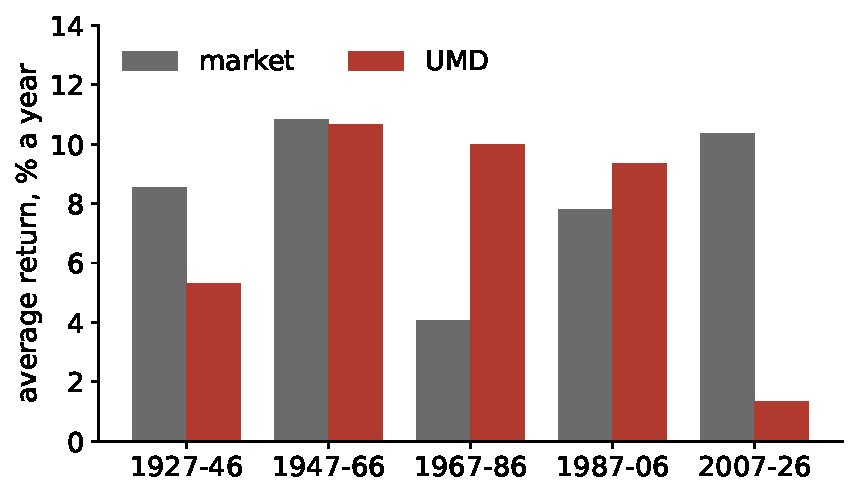
\includegraphics{figures/ca_persist.pdf}}
\vskip 4pt
{\small The market: 4\% to 11\% in every 20 years. But UMD, once published and crowded: 9\% to 1\%. A style factor can behave like an alpha.}
\end{column}
\begin{column}{0.48\textwidth}
\renewcommand{\arraystretch}{1.25}
\begin{tabular}{lc}
\toprule
49 industries & 5 years on next 5 \\
\midrule
correlation of $\alpha$ & \textcolor{red}{$-0.12$} \\
correlation of $\beta$ & $+0.61$ \\
correlation of vol & $+0.75$ \\
\bottomrule
\end{tabular}
\vskip 8pt
\begin{itemize}
\item Our 29: alpha correlates 0.78 across 1980--2000. They are on the list because they worked.
\vskip 4pt
\item After publication, such returns fall 58\% (McLean and Pontiff 2016)
\end{itemize}
\end{column}
\end{columns}
\end{frame}

%================================================================== THE SAME FORMULA
\begin{frame}{Your strategy is an alpha bet and a factor bet}
\[ r_{i} \;=\; \alpha_{i} \;+\; \beta_{i}\,f \;+\; \varepsilon_{i} \]
{\small $r_{i}$: your strategy \qquad $f$: the factor, here the market \qquad $\varepsilon_{i}$: what is left}
\vskip 12pt
Hedge out the factor and trade what is left:
\[ h_{i} \;=\; r_{i} - \beta_{i}\,f \qquad \text{mean } \alpha_{i}, \quad \text{volatility } \sigma_{\varepsilon,i}, \quad \text{no market exposure} \]
\vskip 6pt
\begin{itemize}
\item Anyone can buy the market for free. The hedged piece is what you are sizing here.
\vskip 6pt
\item So the assets become the $h_{i}$, the means become $\alpha_{i}$, and the covariance becomes $\Sigma_{\varepsilon}$
\end{itemize}
\end{frame}

\begin{frame}{Where the inverse disappears}
If the residuals are uncorrelated, $\Sigma_{\varepsilon}$ is diagonal, and inverting it just divides:
\[ W^{\star} \propto \Sigma_{\varepsilon}^{-1}\alpha \qquad\Longrightarrow\qquad w_{i} \propto \frac{\alpha_{i}}{\sigma_{\varepsilon,i}^{2}} \]
Multiply by $\sigma_{\varepsilon,i}$ to get the volatility you give strategy $i$:
\vskip 10pt
\begin{beamercolorbox}[rounded=true,sep=8pt,center]{box1}
$\displaystyle \underbrace{w_{i}\,\sigma_{\varepsilon,i}}_{\text{volatility you give it}} \;\propto\; \underbrace{\frac{\alpha_{i}}{\sigma_{\varepsilon,i}}}_{\text{its appraisal ratio}}$
\end{beamercolorbox}
\vskip 10pt
\begin{itemize}
\item No matrix. The number you have computed since \emph{Performance Evaluation} is a position size.
\vskip 4pt
\item If they are correlated it is the same formula, with the whole matrix: $W^{\star} \propto \Sigma_{\varepsilon}^{-1}\alpha$
\end{itemize}
\end{frame}

\begin{frame}{Bigger alpha does not mean a bigger position}
\vskip 8pt
\begin{center}
\renewcommand{\arraystretch}{1.4}
\begin{tabular}{lccccc}
\toprule
 & $\alpha$ & $\sigma_{\varepsilon}$ & appraisal ratio & weight $\alpha/\sigma_{\varepsilon}^{2}$ & volatility you give it \\
\midrule
Strategy A & 4\% & 4\% & 1.0 & \textcolor{red}{25} & \textcolor{red}{1.0} \\
Strategy B & 8\% & 16\% & 0.5 & 3 & 0.5 \\
\bottomrule
\end{tabular}
\end{center}
\vskip 14pt
\begin{itemize}
\item B has twice the alpha and gets half the risk, and an eighth of the weight
\vskip 8pt
\item The formula divides by a square, so it loves whatever looks \textcolor{red}{quiet}
\end{itemize}
\end{frame}

\begin{frame}{What is combining worth?}
\vskip 14pt
\begin{center}
{\large You run two strategies. Each has a Sharpe ratio of 1.0.\\[4pt] Their correlation is zero. You size them optimally.}
\vskip 18pt
What is the Sharpe ratio of the two together?
\vskip 18pt
\pollbox{gray}{\textbf{A}\ \ 1.0} \hfill
\pollbox{red}{\textbf{B}\ \ 1.41} \hfill
\pollbox{blue}{\textbf{C}\ \ 2.0}
\end{center}
\end{frame}

\begin{frame}{Correlation is an angle}
\begin{columns}[c]
\begin{column}{0.46\textwidth}
\adjustbox{max width=\textwidth, max height=0.62\textheight}{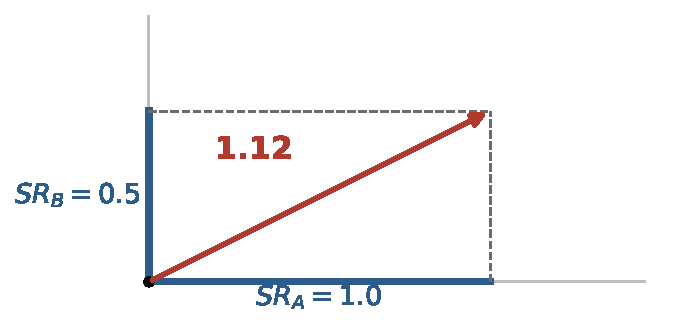
\includegraphics{figures/ca_angle_right.pdf}}
\end{column}
\begin{column}{0.52\textwidth}
\begin{itemize}
\item Draw each strategy as a direction. The angle between two directions has $\cos(\text{angle}) = \rho$.
\vskip 8pt
\item The best combination is a vector, in \textcolor{red}{red}. Its length is the combined Sharpe ratio.
\vskip 8pt
\item Each strategy's Sharpe ratio is the shadow of that vector on its direction
\vskip 8pt
\item Uncorrelated means a right angle, so Pythagoras: $\sqrt{1.0^{2} + 0.5^{2}} = 1.12$
\end{itemize}
\end{column}
\end{columns}
\vskip 10pt
\begin{beamercolorbox}[rounded=true,sep=7pt,center]{box1}
Squared Sharpe ratios add \emph{because} the bets are at right angles
\end{beamercolorbox}
\vskip 2pt
\hfill \hyperlink{appendix_angle}{\beamerbutton{Why}}
\end{frame}

\begin{frame}[label=back_angle]{Change the angle: two strategies, each with a Sharpe ratio of 1}
\begin{center}
\adjustbox{max width=\textwidth, max height=0.56\textheight}{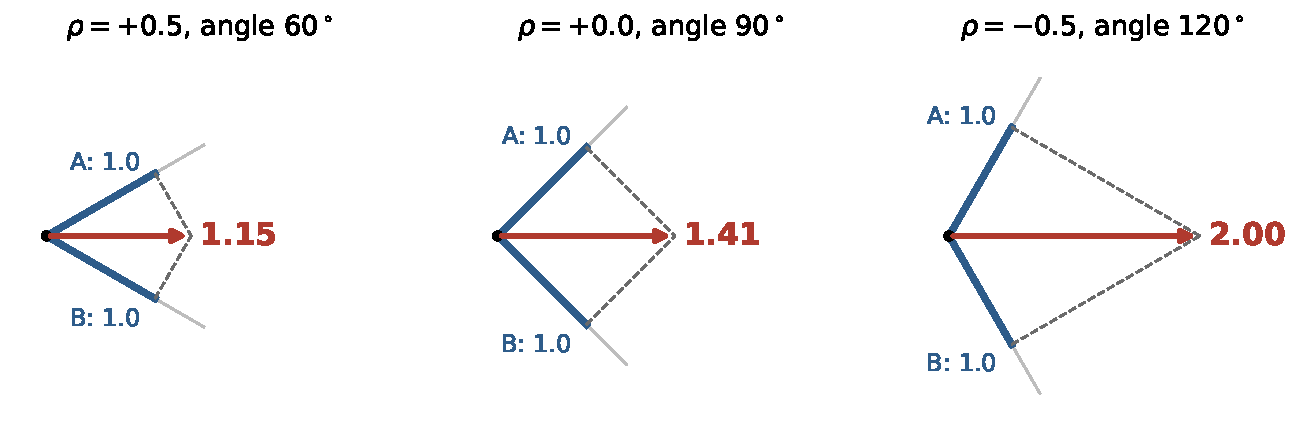
\includegraphics{figures/ca_angle_three.pdf}}
\end{center}
\begin{itemize}
\item \textbf{Positive correlation, under 90$^\circ$:} they overlap: 1.15, less than Pythagoras.
\vskip 2pt
\item \textbf{Negative correlation, over 90$^\circ$:} each one hedges the other: 2.00, more than Pythagoras.
\end{itemize}
\vskip 4pt
\begin{beamercolorbox}[rounded=true,sep=6pt,center]{box1}
Judge a strategy by what it adds to what you hold, not by its Sharpe ratio alone
\end{beamercolorbox}
\end{frame}

%================================================================== WHERE ALPHA COMES FROM
\begin{frame}{The formula needs two inputs. You treat them differently.}
\vskip 4pt
\begin{center}
\renewcommand{\arraystretch}{1.5}
\begin{tabular}{P{2.3cm}P{5.4cm}P{5.0cm}}
\toprule
$\Sigma_{\varepsilon}$ & \textbf{estimate it} & recent data, high frequency \\
\midrule
$\alpha$ & \textbf{a track record} & $\hat\alpha$, with a standard error \\
 & \textbf{a signal} & your signal's forecast, scaled \\
 & \textbf{a view} & a hunch, made into a number \\
\bottomrule
\end{tabular}
\end{center}
\vskip 12pt
\begin{itemize}
\item In practice most of the thinking goes into $\alpha$ and most of the data goes into $\Sigma_{\varepsilon}$
\vskip 6pt
\item The formula cannot tell which $\alpha$ came from where. You have to.
\end{itemize}
\vskip 8pt
\begin{beamercolorbox}[rounded=true,sep=7pt,center]{box1}
Estimate the risk. Supply the alpha.
\end{beamercolorbox}
\end{frame}

\begin{frame}{A hunch is not an input until it is a number}
\vskip 10pt
\begin{itemize}
\item ``I like Apple.'' Compared to what, by how much, by when, and how sure are you?
\vskip 12pt
\item Leaving it out is also a number. It is $\alpha = 0$, and the formula will act on it.
\vskip 12pt
\item Once it is a number it can be sized, combined with your other bets, and \textcolor{red}{scored} when the date arrives
\vskip 12pt
\item Without a number you cannot be wrong, and so you cannot learn. That was \emph{Hiring and Firing}, applied to yourself.
\end{itemize}
\vskip 16pt
\begin{beamercolorbox}[rounded=true,sep=7pt,center]{box1}
The discipline is to write the number down before the event
\end{beamercolorbox}
\end{frame}

\begin{frame}{From a hunch to a number: Apple's earnings will beat consensus}
\vskip 2pt
\begin{center}
\renewcommand{\arraystretch}{1.3}
\small
\begin{tabular}{P{3.2cm}P{6.7cm}c}
\toprule
the question & your answer (stylized) & the number \\
\midrule
What is in the price? & consensus earnings \$1.60; you say \$1.68 & a 5\% beat \\
What is a beat worth? & past 5\% beats moved the stock about 4\%: estimate it & $\pm$4\% \\
How sure are you? & right 60\% of the time; wrong means a miss & $(0.6-0.4)\times 4\%$ \\
By when? & the report is in six weeks, then the edge is gone & 30 trading days \\
How much risk? & 25\% a year of stock-specific volatility: $25\%\sqrt{30/252}$ & 8.6\% \\
\bottomrule
\end{tabular}
\end{center}
\vskip 8pt
\begin{beamercolorbox}[rounded=true,sep=7pt,center]{box1}
$\alpha = +0.8\%$ over six weeks, on Apple hedged for the market and its industry
\end{beamercolorbox}
\vskip 8pt
\begin{itemize}
\item It is not 6.7\% a year. You earn that only if you have another idea like it every six weeks.
\end{itemize}
\end{frame}

\begin{frame}{Check the number: what have you just claimed?}
\vskip 4pt
\begin{center}
\renewcommand{\arraystretch}{1.35}
\begin{tabular}{lcc}
\toprule
 & right 60\% & right 55\% \\
\midrule
$\alpha$ over six weeks & 0.8\% & 0.4\% \\
$\alpha/\sigma$ over six weeks: the IC you are claiming & \textcolor{red}{0.09} & 0.05 \\
appraisal ratio, a year & 0.27 & 0.13 \\
position, in a 10\%-volatility book with Sharpe ratio 1 & 11\% & \textcolor{red}{5\%} \\
\bottomrule
\end{tabular}
\end{center}
\vskip 10pt
\begin{itemize}
\item Good managers run an IC of about 0.02 to 0.05 (Grinold and Kahn). Is this the best idea you have ever had?
\vskip 6pt
\item Position: volatility given $= (AR/SR_{\text{book}})\times 10\%$, so the weight is that over 25\%
\vskip 6pt
\item Being honest about your confidence halved the position. That is the formula working.
\end{itemize}
\end{frame}

\begin{frame}[label=back_bl]{A taste of Black--Litterman: start from no alpha, add your views}
\begin{columns}[c]
\begin{column}{0.56\textwidth}
\adjustbox{max width=\textwidth, max height=0.66\textheight}{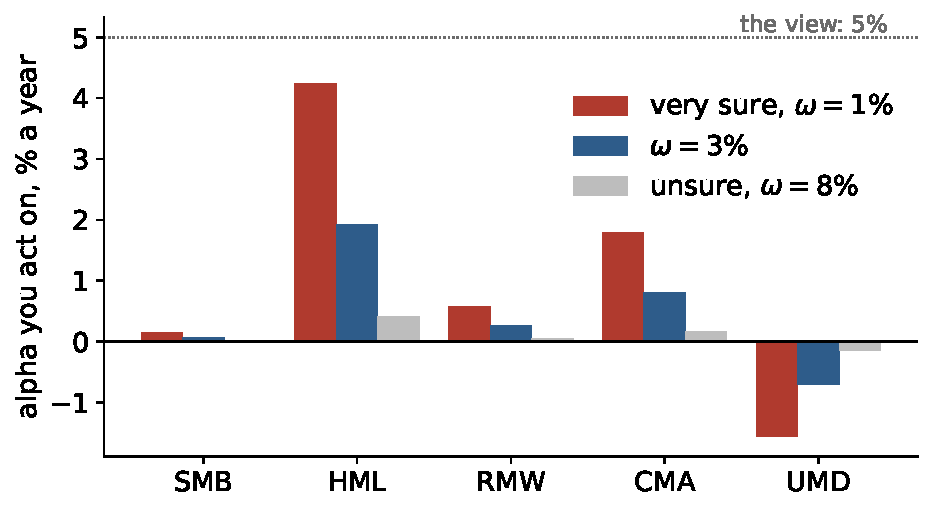
\includegraphics{figures/ca_bl.pdf}}
\end{column}
\begin{column}{0.42\textwidth}
\[ \alpha_{\text{act}} \;=\; \frac{\tau^{2}}{\tau^{2}+\omega^{2}}\;\alpha_{\text{view}} \]
{\small $\tau$: how big alphas tend to be. \\ $\omega$: your view's standard error.}
\vskip 8pt
\begin{itemize}
\item One view: HML's alpha is 5\%
\vskip 5pt
\item Less sure, smaller bet
\vskip 5pt
\item Its neighbours' alphas move too, CMA up and UMD down, and that is why you end up holding only HML
\end{itemize}
\end{column}
\end{columns}
\vskip 6pt
\begin{beamercolorbox}[rounded=true,sep=6pt,center]{box1}
Your alpha is an estimate, so shrink it. That is \emph{Capital Allocation III} in one line.
\end{beamercolorbox}
\vskip 1pt
\hfill \hyperlink{appendix_bl}{\beamerbutton{The whole formula}}
\end{frame}

\begin{frame}{Now: the notebook}
\vskip 2pt
\begin{beamercolorbox}[rounded=true,sep=7pt,center]{box1}
\textbf{Notebook: Capital Allocation II} \ --- \ the same formula, on hedged portfolios
\end{beamercolorbox}
\vskip 8pt
\begin{enumerate}
\item \textbf{Alpha bets on five factors.} Hedge, size, build the book, combine it with the market.
\vskip 4pt
\item \textbf{All 29 strategies.} The rule against the whole matrix. Look at the positions.
\vskip 4pt
\item \textbf{Your views.} Put one number in, and watch the book move.
\end{enumerate}
\vskip 6pt
{\small \textbf{Bring back:} the Sharpe ratio of your book, of the market, and of the two together. Does the formula hold? \\[2pt]
Stop at \textbf{Back to the slides}; the challenge after it is homework.}
\end{frame}

%================================================================== BREADTH
\begin{frame}{0.57 and 0.97 make 1.12}
\vskip 4pt
\begin{center}
\renewcommand{\arraystretch}{1.3}
\begin{tabular}{lc}
\toprule
 & Sharpe ratio, 1980--2026 \\
\midrule
the market & 0.57 \\
the book: five factors, hedged, sized by the rule & 0.97 \\
the two together & \textcolor{red}{1.12} \\
$\sqrt{0.57^{2} + 0.97^{2}}$ & \textcolor{red}{1.12} \\
\midrule
the book, if its five pieces were uncorrelated & 1.10 \\
\bottomrule
\end{tabular}
\end{center}
\vskip 8pt
\begin{itemize}
\item The hedge makes the book uncorrelated with the market, so the formula is exact
\vskip 6pt
\item Inside the book it falls short: 0.97, not 1.10. HML and CMA are correlated 0.66.
\end{itemize}
\vskip 6pt
\begin{center}
So: how much does correlation cost when you have many bets?
\end{center}
\end{frame}

\begin{frame}{Why pod shops exist}
\[ SR_{\text{pool}} \;=\; \sqrt{N}\times SR_{\text{pod}} \]
{\small $N$ uncorrelated teams, each hedged, each with the same Sharpe ratio. The last formula, with $N$ terms.}
\vskip 14pt
\begin{itemize}
\item A pod with a Sharpe ratio of 0.5 is not a fund. Nobody allocates to it.
\vskip 8pt
\item Thirty of them, uncorrelated, make \textcolor{red}{2.7}. That is one of the best records in the industry.
\vskip 8pt
\item Citadel and Millennium run many small hedged teams, each on its own risk budget
\end{itemize}
\vskip 14pt
\begin{beamercolorbox}[rounded=true,sep=7pt,center]{box1}
The pods are worth more together than apart, and that gap is the firm
\end{beamercolorbox}
\end{frame}

\begin{frame}[label=appendix_pool_back]{Our 29 strategies: 0.40 apart, 1.38 together}
\begin{columns}[c]
\begin{column}{0.58\textwidth}
\adjustbox{max width=\textwidth, max height=0.68\textheight}{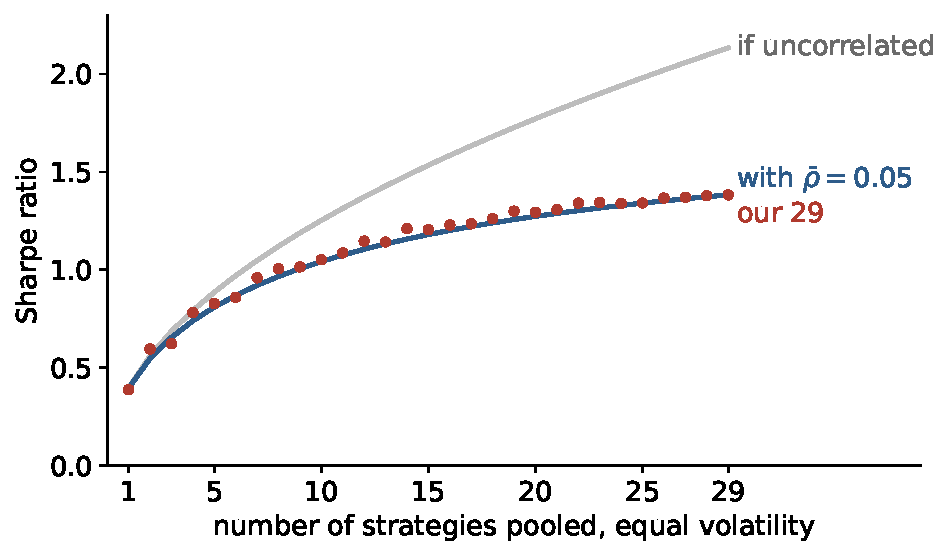
\includegraphics{figures/ca_pool.pdf}}
\end{column}
\begin{column}{0.40\textwidth}
\begin{itemize}
\item $\sqrt{29}\times 0.40 = 2.13$. We get 1.38.
\vskip 6pt
\item The whole gap is correlation:
\[ \bar{s}\,\sqrt{\frac{N}{1+(N-1)\bar\rho}} \;=\; 1.38 \]
\item $\bar\rho$ is only 0.05. Even with endless strategies you stop at \textcolor{red}{1.78}.
\end{itemize}
\vskip 2pt
\hfill \hyperlink{appendix_pool}{\beamerbutton{Why}}
\end{column}
\end{columns}
\vskip 8pt
\begin{beamercolorbox}[rounded=true,sep=6pt,center]{box1}
The scarce thing is not a good strategy. It is an uncorrelated one.
\end{beamercolorbox}
\end{frame}

\begin{frame}{One result, three forms: skill times breadth}
\vskip 8pt
\begin{center}
\renewcommand{\arraystretch}{1.5}
\begin{tabular}{ll}
\toprule
two uncorrelated bets & $SR = \sqrt{SR_{A}^{2} + SR_{B}^{2}}$ \\
$N$ pods & $SR_{\text{pool}} = \sqrt{N}\;SR_{\text{pod}}$ \\
the Fundamental Law (Grinold 1989) & $IR = IC\times\sqrt{\text{breadth}}$ \\
\bottomrule
\end{tabular}
\end{center}
\vskip 10pt
{\small $IC$: the correlation between your forecasts and what happened. Breadth: independent bets a year.}
\vskip 12pt
\begin{itemize}
\item $IC = 0.03$ is barely detectable. With 1,000 independent bets a year, $IR \approx$ \textcolor{red}{0.95}.
\vskip 6pt
\item It names the pattern you just derived twice, and it is the IC you claimed for Apple.
\end{itemize}
\end{frame}

\begin{frame}{The catch}
\begin{columns}[c]
\begin{column}{0.56\textwidth}
\adjustbox{max width=\textwidth, max height=0.64\textheight}{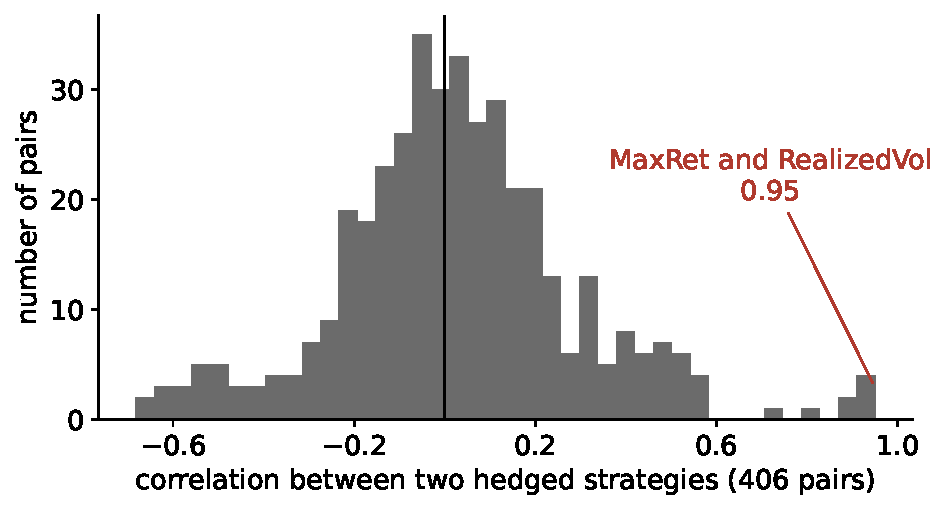
\includegraphics{figures/ca_resid_corr.pdf}}
\end{column}
\begin{column}{0.42\textwidth}
\begin{itemize}
\item Average correlation 0.03. It looks like zero.
\vskip 8pt
\item Average \emph{absolute} correlation \textcolor{red}{0.20}
\vskip 8pt
\item Some pairs are one trade under two names
\end{itemize}
\end{column}
\end{columns}
\vskip 10pt
\begin{beamercolorbox}[rounded=true,sep=7pt,center]{box1}
Every formula so far assumed you know $\mu$ and $\Sigma$. You estimated them. \\
\emph{Capital Allocation III}: what that costs.
\end{beamercolorbox}
\end{frame}

\begin{frame}{Now you: four ideas, before you look at any data}
Using the 49 industries, each idea is a hedged long-short. Discuss, then write them down:
\vskip 8pt
\begin{itemize}
\item \textbf{What do you think you know?} AI spending, interest rates, oil, an aging population, a recession.
\vskip 6pt
\item \textbf{Why is it not in the price?} If you cannot say, your alpha is zero.
\vskip 6pt
\item \textbf{By when, and how sure?} Then one number for each.
\vskip 6pt
\item \textbf{Are they four ideas?} Two that are correlated 0.9 are one idea.
\end{itemize}
\vskip 12pt
\begin{beamercolorbox}[rounded=true,sep=7pt]{box1}
\textbf{Homework: four trading ideas.} Write the number first. Then estimate the risk, look at the record, shrink, and size the book. The memo defends your biggest position.
\end{beamercolorbox}
\end{frame}

\begin{frame}{Takeaways}
\begin{enumerate}
\item Factor bets interact with your life, so tilt them. True alpha does not, so maximize the Sharpe ratio.
\vskip 5pt
\item A factor's mean is slow and an alpha decays. Long history for one, signals and judgment for the other.
\vskip 5pt
\item It is the same formula on hedged portfolios. Without correlation, volatility follows the appraisal ratio.
\vskip 5pt
\item Correlation is an angle: under 90$^\circ$ adds less than Pythagoras, over 90$^\circ$ adds more.
\vskip 5pt
\item Estimate the risk, supply the alpha, and write the number down before the event.
\vskip 5pt
\item Breadth is the prize, and correlation limits it: 0.40 apart, 1.38 together, not 2.13.
\end{enumerate}
\end{frame}

%================================================================== APPENDIX
\appendix
\begin{frame}
\begin{center}
{\Large Appendix}
\end{center}
\end{frame}

\begin{frame}[label=appendix_angle]{A: Why the picture is exact}
Two strategies with Sharpe ratios $s_{1},s_{2}$ and correlation $\rho$. The best combination has
\[ SR^{2} \;=\; \frac{s_{1}^{2} + s_{2}^{2} - 2\rho\, s_{1}s_{2}}{1-\rho^{2}} \]
\vskip 4pt
\begin{itemize}
\item Any asset's Sharpe ratio equals the best Sharpe ratio times its correlation with the best portfolio: $s_{i} = SR\,\rho_{i,\star}$
\vskip 6pt
\item That is the shadow: $SR\cos(\text{angle})$. The red vector is the one whose two shadows are $s_{1}$ and $s_{2}$.
\vskip 6pt
\item With $s_{1}=s_{2}=s$: $SR = s\sqrt{2/(1+\rho)}$, so $1.15s$, $1.41s$, $2s$ at $\rho = 0.5, 0, -0.5$
\vskip 6pt
\item If $s_{2}/s_{1} < \rho$, the red vector falls outside the two directions: a short position, as in \emph{Capital Allocation III}
\end{itemize}
\hfill \hyperlink{back_angle}{\beamerreturnbutton{Back}}
\end{frame}

\begin{frame}[label=appendix_bl]{A: Black--Litterman, the whole formula}
\[ \alpha_{\text{act}} \;=\; \pi \;+\; \tau\Sigma P'\,\big(P\,\tau\Sigma\, P' + \Omega\big)^{-1}\big(Q - P\pi\big) \]
\vskip 4pt
{\small $\pi$: the prior; for hedged bets, zero. \quad $\tau\Sigma$: the prior's covariance; here $\tau = 0.05$. \\
$P$: which portfolios your views are on. \quad $Q$: the numbers. \quad $\Omega$: how unsure you are.}
\vskip 10pt
\begin{itemize}
\item One view on one asset: $P$ picks it out, and the first term becomes $\tau^{2}/(\tau^{2}+\omega^{2})$ with $\tau^{2}=\tau\sigma^{2}$
\vskip 6pt
\item The $\Sigma$ in front moves every asset correlated with your view. Then $\Sigma^{-1}\alpha_{\text{act}}$ cancels it: with $\pi=0$ the weights are a multiple of $P'$, so you hold only what you have a view on
\vskip 6pt
\item In the original, $\pi$ comes from the market's weights, so with no views you hold the market (Black and Litterman 1992)
\end{itemize}
\hfill \hyperlink{back_bl}{\beamerreturnbutton{Back}}
\end{frame}

\begin{frame}[label=appendix_pool]{A: Why correlation sets the limit}
Scale $N$ strategies to the same volatility $\sigma$, and hold them equally. Let $\bar{s}$ be their average Sharpe ratio and $\bar\rho$ their average pairwise correlation.
\vskip 8pt
\[ \text{mean of the pool} = \bar{s}\,\sigma \qquad\qquad
   \text{variance of the pool} = \frac{\sigma^{2}}{N}\Big(1 + (N-1)\bar\rho\Big) \]
\vskip 6pt
\[ SR_{\text{pool}} \;=\; \bar{s}\,\sqrt{\frac{N}{1+(N-1)\bar\rho}} \;\;\xrightarrow{\;N\to\infty\;}\;\; \frac{\bar{s}}{\sqrt{\bar\rho}} \]
\vskip 6pt
\begin{itemize}
\item This is an identity, not an approximation, which is why it matches the 29 to three decimals
\vskip 6pt
\item $\bar\rho = 0$ gives back $\sqrt{N}\,\bar{s}$
\vskip 6pt
\item In the figure, each red dot averages 300 random sets of $N$ strategies
\end{itemize}
\hfill \hyperlink{appendix_pool_back}{\beamerreturnbutton{Back}}
\end{frame}

\begin{frame}{A: Data, and what to be careful about}
\begin{itemize}
\item \textbf{Six factors.} Ken French: market, SMB, HML, RMW, CMA, UMD. Monthly, 1980--2026, 558 months. UMD and the 49 industries go back to 1927.
\vskip 8pt
\item \textbf{The 29 strategies.} Long-shorts on published signals, on our CRSP panel, 1980--2000, 251 months.
\vskip 8pt
\item \textbf{Selection.} These signals are in the literature because they worked, much of it in this sample. Their Sharpe ratios are overstated as forecasts of what comes next.
\vskip 8pt
\item \textbf{In sample.} Alphas, betas and residual volatilities use the full period. Every Sharpe ratio built from them is in sample, and so is every book.
\vskip 8pt
\item \textbf{The Apple numbers are stylized.} Estimate the response to a surprise before you use it.
\end{itemize}
\end{frame}

\end{document}
